\documentclass[12pt]{beamer}
\usetheme{Copenhagen}
\usepackage[utf8]{inputenc}
\usepackage{hyperref}
\newcommand{\tmop}[1]{\ensuremath{\operatorname{#1}}}
\beamertemplatenavigationsymbolsempty

\title[Stereo matting]{Stereo matting by image warping}
\subtitle{Advanced Methods for Computer Vision}
\author{François-Xavier Thomas}
\institute{ENS Cachan}
\date{March 31, 2012}

\AtBeginSection[]
{
  \begin{frame}{Outline}
  \tableofcontents[currentsection]
  \end{frame}
}

\begin{document}

\begin{frame}
\titlepage
\end{frame}

\section{Introduction}

\begin{frame}{Disclaimer}
  \begin{itemize}
    \item The aim of this presentation is to introduce the paper \emph{A Stereo Approach that Handles the Matting Problem via Image Warping}, by Michael Bleyer et al.
    \item I won't delve into the details here, but you can find them, along with the source code, on my \textbf{GitHub} repository :
    \center{\footnotesize\color{blue} \url{http://github.com/fxthomas/mva-advancedcv-project/}}
  \end{itemize}
\end{frame}

\begin{frame}{Introduction}
  \begin{block}{WarpMat}
    The \emph{WarpMat} algorithm described in this paper is a stereo vision method for the computation of a multilayered matting segmentation of the scene.
  \end{block}

  \begin{block}{Properties}
    \begin{itemize}
      \item \textbf{Matting} is the decomposition of the image into multiple planes (foreground, background, ...)
      \item Matting involves computation of the \textbf{opacity} at the border of each layer $\Rightarrow$ better \textbf{color blending}
      \item \textbf{Multilayered}: Unlike other algorithms, not only foreground and background layers
    \end{itemize}
  \end{block}
\end{frame}

\section{Algorithm initialization}

\begin{frame}{Algorithm initialization}
  \begin{block}{Energy minimization}
    \begin{itemize}
      \item \emph{WarpMat} is an \textbf{energy minimization} algorithm
      \item To converge, it needs reasonably good guesses as initial values
    \end{itemize}
  \end{block}

  \begin{block}{Initial requirements}
    \begin{itemize}
      \item Rectified images
      \item A disparity map
      \item An over-segmentation of the left view
    \end{itemize}
  \end{block}
\end{frame}

\subsection{Image rectification}

\begin{frame}{Image rectification}
  \begin{block}{}
    \begin{itemize}
      \item As a stereo vision algorithm, we need \textbf{rectified images} for the left and right views.
      \item We can then only follow a single scanline to search for the disparities
    \end{itemize}

  \end{block}
  \begin{center} 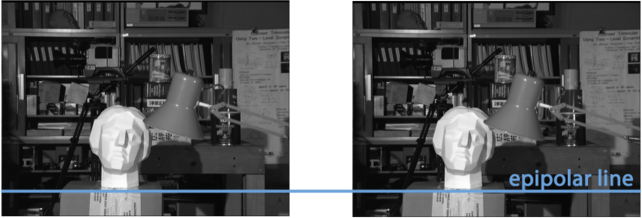
\includegraphics[height=3cm]{../images/Rectify-Scanlines.png} \end{center}
\end{frame}

\subsection{Disparity map}

\begin{frame}{Disparity map}
  \begin{block}{}
    The authors of \emph{WarpMat} recommend a specific method for the computation of the disparity map, called \emph{SimpleTree}, which yields pretty good results.
  \end{block}
  \begin{center} 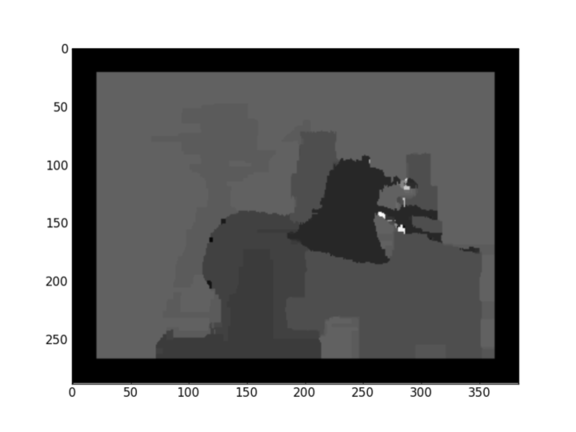
\includegraphics[height=5cm]{../images/Disparity-Tsukuba.png} \end{center}
\end{frame}

\begin{frame}{The return of the disparity map}
  \begin{block}{}
    \emph{SimpleTree} also yields relatively homogeneous disparity maps, even in very bad conditions.
  \end{block}

  \begin{center} 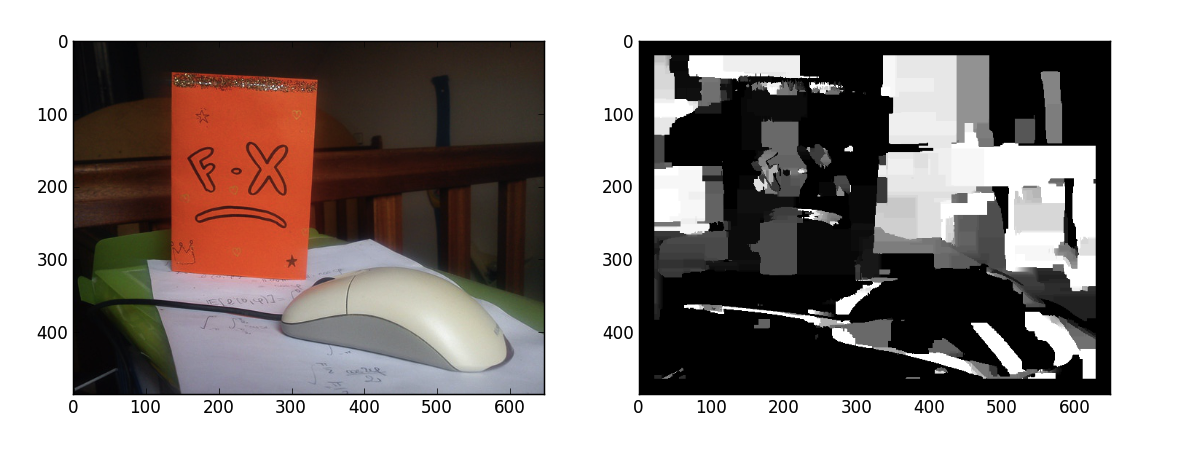
\includegraphics[height=4cm]{../images/Disparity-FX-Both.png} \end{center}
\end{frame}

\begin{frame}{Message passing}
  \begin{block}{Energy minimization}
    \emph{SimpleTree} is based on, guess what? Energy minimization!

    \footnotesize
    \[ E \left( D \right) = E_{\tmop{data}} \left( D \right) +
       E_{\tmop{smoothness}} \left( D \right) = \sum_{p \in \mathcal{P}}
       \underbrace{m \left( p, d_p \right)}_{\text{cost of $d_p$}} + \sum_{\left(
       p, q \right) \in \mathcal{N}} \underbrace{s \left( d_p, d_q
       \right)}_{\text{closeness}} \]
  \end{block}

  \begin{block}{How to optimize?}
    \begin{itemize}
      \item Fully connected graph
      \item Tree-based DP
      \item \emph{SimpleTree}
    \end{itemize}
  \end{block}
\end{frame}

\begin{frame}{Message passing}
  \begin{block}{Fully connected graph}
    \begin{itemize}
      \item Every pixel is connected to its neighbors $\Rightarrow$ \textbf{complexity}
      \item Cyclic graph $\Rightarrow$ \textbf{approximate} message passing
    \end{itemize}

    \begin{center}
      \includegraphics[height=4cm]{graphics/disparity-wholetree.eps}
    \end{center}
  \end{block}
\end{frame}

\begin{frame}{Message passing}
  \begin{block}{Tree-based DP}
    \begin{itemize}
      \item Exact minimization in two passes (\textbf{forward-backward})
      \item Reduced complexity
    \end{itemize}
  \end{block}

  \begin{center}
    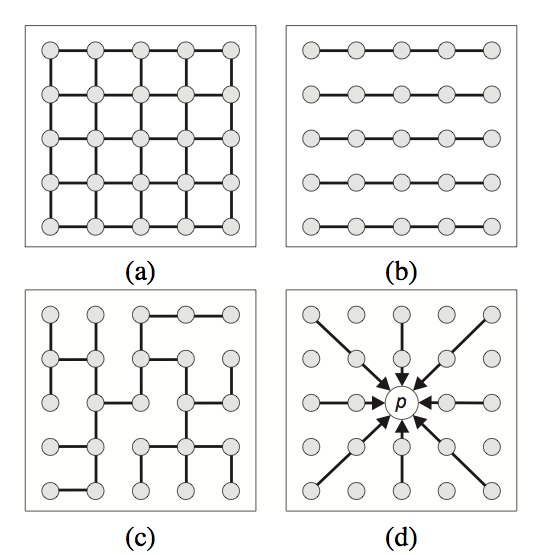
\includegraphics[height=4cm]{../images/Tree-DP.png}
  \end{center}
\end{frame}

\begin{frame}{Message passing}
  \begin{block}{\emph{SimpleTree}}
    \begin{itemize}
      \item Still tree-based, still \textbf{exact}
      \item \textbf{Separate} minimization : first horizontally, then vertically
      \item This minimization and a rotated tree reduce artifacts
    \end{itemize}
  \end{block}

  \begin{center}
    \includegraphics[height=4cm]{graphics/disparity-simpletree.eps}
  \end{center}
\end{frame}

\begin{frame}{Implementation}
  \begin{block}{Core DP pass}
    \begin{itemize}
      \item The way individual horizontal scanlines are brought together in the vertical optimization is exactly the same as the horizontal optimization.
      \item Together, all these optimizations are the result of 8 passes over different axes of the image : the same method is called each time!
    \end{itemize}
  \end{block}

  \begin{block}{Performance}
    \begin{itemize}
      \item For a Tsukuba ($380 \times 288$) image pair, approx. 1.5s
      \item For a $648 \times 486$ image pair, approx. 7s
    \end{itemize}
  \end{block}
\end{frame}

\subsection{Segmentation}

\begin{frame}{Mean-Shift Segmentation}

\end{frame}

\end{document}
